% 09-exotics — the tetraquark/hexaquark search; no 1990 counterpart
\section{Tetraquark and hexaquark candidates}
\label{sec:exotics}

The 1990 paper met multiquark states twice without pursuing them: the
$\pi\pi$-continuum meson state of its Fig.~5(d) and the two-baryon state of
its Fig.~6(d).  This section pursues them.  Large-$N$ analyses of
meson--meson scattering predict a tetraquark pole very close to the lowest
two-meson threshold~\cite{Sazdjian:2025mqg,Sazdjian:2024vlm,Lucha:2017gqq,
Chen:2019dbk}, and tensor-network studies at finite density find
multibaryon bound states of striking robustness~\cite{Silvi:2016cas,
Silvi:2019wnf}.  Both claims are testable here at finite $N$, in the
original quantization, with controlled resolution systematics.

Three diagnostics run over every level of the $B=0$ and $B=2$ spectra.
The Fock-sector weight, computed exactly from the block-diagonal norm,
classifies each state by its dominant parton number; a tetraquark
candidate is a level whose four-parton weight exceeds one half, not a
level number chosen by eye.  The binding energy is a same-$K$ correlated
difference, $\Delta = M - 2M_{\rm thresh}$, with state and threshold on
one grid; the analysis code refuses any other construction, since
differencing two separate extrapolations double-counts every shared
systematic.  And the drift of $\Delta$ with resolution separates the two
hypotheses: a discretization artifact runs with the grid, a bound state
does not.  At $N=4$ the meson, baryon, and $B=2$ sectors share even
$K_{\rm code}$, so exact same-$K$ differences exist for every threshold;
at $N=3$ the baryon grid is odd, and the two-baryon study runs at $N=4$
for exactly that reason.

\begin{figure*}
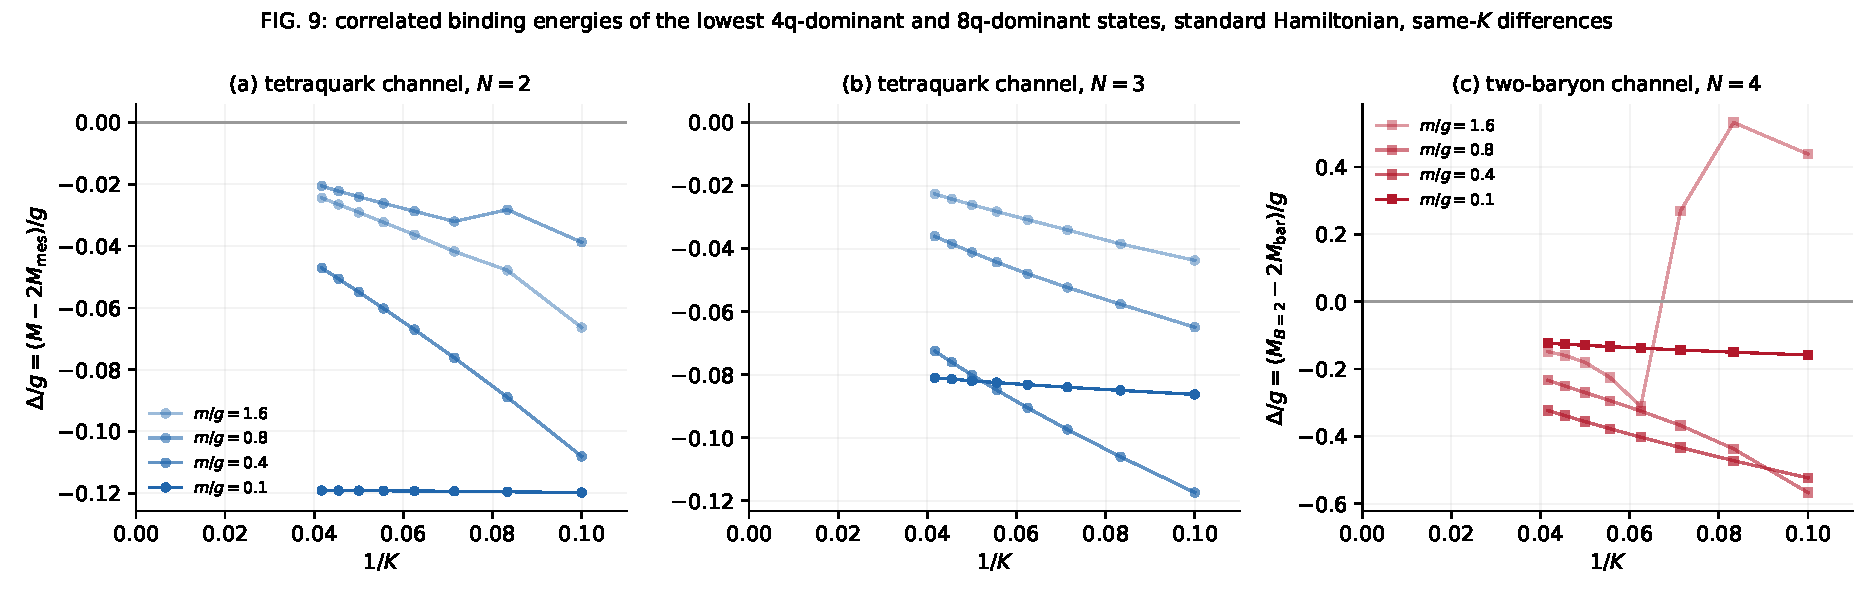
\includegraphics[width=\textwidth]{figs/fig9_exotics.pdf}
\caption{Correlated binding energies against $1/K$, standard Hamiltonian,
even $2K = 20$--$48$, Fock truncations $\mathrm{LPN} = 6$ ($B=0$, $N=2,3$)
and $10/6$ ($B=2/B=1$, $N=4$), $m/g$ as labeled, no fits drawn.  (a), (b):
lowest four-quark-dominant $B=0$ level minus twice the same-$K$ meson
mass.  (c): $B=2$ ground state minus twice the same-$K$ baryon mass.  The
$m/g=1.6$ discontinuity in (c) is a level crossing, discussed in the
text.}
\label{fig:exotics}
\end{figure*}

Figure~\ref{fig:exotics} shows both channels.  The pattern splits cleanly
by coupling.  At weak coupling the four-quark deficit drains away with
resolution: extrapolated in $1/K$, the $N=2$ channel gives
$\Delta/g = \numExoTetraNTwoMgOnepSix$ at $m/g = 1.6$, consistent with
zero.  The $N=3$ channel gives $\numExoTetraNThreeMgOnepSix$: a
threshold-hugging whisper, two to three spreads below zero, precisely the
regime where the large-$N$ scattering analyses place their near-threshold
pole.  We flag it as a candidate and decline to claim it; the quoted
spread is a fit-ensemble width, not a full budget.

Strong coupling is different in kind.  At $m/g = 0.1$ the lowest
four-quark-majority level sits below twice the meson mass by
$\numExoTetraNTwoMgZeropOne$ at $N=2$ and
$\numExoTetraNThreeMgZeropOne$ at $N=3$, and the deficit does not move:
it is flat in $1/K$ at the fourth decimal across a factor of 2.4 in
resolution.  By the drift criterion this is a converged sub-threshold
state.  What it is a state \emph{of} is less clean, and we state the
mixing plainly: its four-quark weight is 0.5--0.7, not 0.99, so it is a
strongly mixed object rather than a compact tetraquark, and at this
coupling the distinction between ``bound two-meson molecule'' and
``four-quark state'' may not survive scrutiny.  The massless limit
enforces $\Delta \to 0$ at $m/g \to 0$ (Sec.~\ref{sec:massless}), so the
binding must eventually release; mapping where sits beyond this first
survey.

The two-baryon channel echoes the tensor-network finding.  The $N=4$
$B=2$ ground state is structurally a hexaquark --- its eight-parton Fock
weight is \numHexaEightqWeight{} at $2K=48$, $m/g=0.1$ --- and it sits
below twice the baryon mass at every resolution reached, with
$\Delta/g = \numExoHexaMgZeropOne$ at $m/g = 0.1$ and
$\numExoHexaMgZeropFour$ at $0.4$.  At $m/g = 1.6$ the channel changes
character between $2K = 28$ and $32$: the correlated difference jumps
sign, the signature of a level crossing in one of the sectors, and we
exclude the pre-crossing points from the fit and quote
$\numExoHexaMgOnepSix$ with its accordingly useless spread.  Identifying
which levels cross, and whether the weak-coupling channel binds at all,
needs the crossing resolved rather than averaged over.

Two closing caveats bound this section's claims.  All of it is
standard-Hamiltonian physics at couplings above the validity boundary of
Sec.~\ref{sec:budget}, where that Hamiltonian is reliable; none of it
extrapolates into the chiral region.  And every binding energy here is a
statement about this theory's spectrum at finite $N$, not yet matched to
the unitarized large-$N$ amplitudes it was motivated by; that comparison
needs the scattering normalization those analyses use, and we leave it as
the natural next step.

% \itodo{NF=2 manifestly-exotic channels (Python-only capability) — the
% flavor-nonsinglet probe runs; a v2 candidate if time allows.}
